\fancyhead[C]{Section 16.7}
	\fancyhead[R]{\daytwentysix}
	
\iftoggle{questions}{
\begin{center}{\large \textbf{Math 2551 Worksheet: Stokes' Theorem}}
\end{center}
\title{Math 2551 Worksheet: Stokes' Theorem}

\begin{enumerate}

\item Let $H$ be the hemisphere and $P$ be the portion of a paraboloid shown below. Use Stokes' Theorem to explain why, if $\bF$ is a vector field on $\R^3$ whose components have continuous partial derivatives, we must have \[\iint_H (\nabla \times \bF) \dotp \bn\ d\sigma=\iint_P (\nabla \times \bF) \dotp \bn\ d\sigma .\]

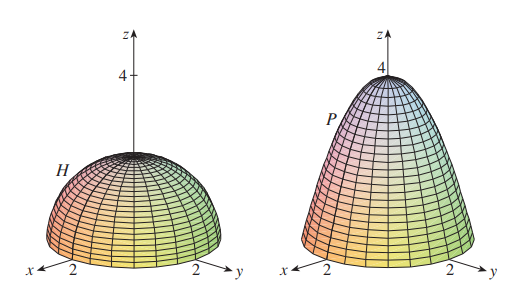
\includegraphics[scale=0.8]{ws_27_ph.png}

\item Use Stokes' Theorem to evaluate $\iint_S (\nabla \times \bF)\dotp \bn\ d\sigma$, where $\bF=\langle x^2z^2,y^2z^2,xyz\rangle$ and $S$ is the part of the paraboloid $z=x^2+y^2$ that lies inside the cylinder $x^2+y^2=4$, oriented upward.

\item A particle moves along line segments from the origin to the points $(1,0,0), (1,2,1),(0,2,1)$, and back to the origin under the influence of the force field
\[\bF(x,y,z)=z^2\bi+2xy\bj+2y^2\bk. \]
Find the work done by the field on the particle.
\end{enumerate}
}{}

\iftoggle{answers}
{
	\begin{center}{\large \textbf{Math 2551 Worksheet Answers: Stokes' Theorem}}
	\end{center}
	
	
	\begin{enumerate}
		
		\item $H$ and $P$ have the same oriented boundary curve $C$ provided that they are oriented in the same way, so by Stokes' theorem the given integrals must be equal.
		
		\item 0
		
		\item 3
	\end{enumerate}

}{}
\iftoggle{solutions}
{
Solutions go here in the same format.
}{}
